\documentclass[11pt,a4paper]{article}

\usepackage[T1]{fontenc}
\usepackage[utf8]{inputenc}
\usepackage[english]{babel}
\usepackage{mathpazo}
\usepackage[margin=2.6cm]{geometry}
\usepackage[expansion=false]{microtype}
\usepackage{booktabs}
\usepackage{array}
\usepackage{longtable}
\usepackage{xcolor}
\usepackage{pgfplots}
\pgfplotsset{compat=1.16}
\usepackage{setspace}
\usepackage{enumitem}
\usepackage{url}
\usepackage[hidelinks]{hyperref}
\usepackage{caption}

\makeatletter
\g@addto@macro\UrlBreaks{\do\-\do\.\do\/\do\_}
\makeatother

\emergencystretch=4em

\definecolor{accent}{HTML}{0B6E6E}
\definecolor{muted}{HTML}{6B7280}

\newcommand{\paperauthor}{Leonardo Covarrubias Garc\'ia}
\setstretch{1.08}
\setlength{\parskip}{0.55em}
\setlength{\parindent}{0pt}
\captionsetup{font=small,labelfont=bf}

\title{\textbf{Measure Before You Automate}\\[0.3em]
\large A Reading of the \emph{AI Playbook for Finance 2027} from the Mexican Context}
\author{\paperauthor\\[0.35em]
  {\normalsize\color{muted}AI-Native Economist}}
\date{October 2026}

\begin{document}
\maketitle

\begin{abstract}
\noindent
Paystand, a B2B payments platform, has published an artificial intelligence playbook for finance leaders in Mexico. This text reads it with three questions: which of its figures survive verification, which tensions its argument conceals, and what all of it means for a Mexican company. Of thirteen claims checked against public sources, seven are confirmed outright, two with reservations, one arithmetic example is correct, and three could not be fully confirmed or need qualification. The central finding is this: 71\% of finance leaders perceive that AI meets their return expectations, yet only 7\% of organizations, in Mexico as in the world, have consolidated that return. The distance between the two figures is the distance between perceiving and measuring. The text closes with five practical principles and a set of questions for evaluating any vendor.
\end{abstract}

\section{Introduction}

Every new discipline passes through a stage in which enthusiasm outruns measurement. Artificial intelligence applied to corporate finance is in that moment now: announcements of adoption abound, while proof of return is scarce. The \emph{Playbook de IA para finanzas 2027} (``AI Playbook for Finance 2027'')~\cite{paystand} enters at exactly that point with a sober thesis, which can be summarized in its own words: what separates the 7\% that consolidated their return from everyone else is not the model, but having measured before starting.

This text is a reading, not primary research. No figure in it is original: all come from the playbook or from the public sources cited, and Section~\ref{sec:limits} details what was consulted first-hand and what only through specialized press. The reading is made from Mexico because the document is addressed to Mexican finance directors, and because the local environment (the SAT tax authority, the CFDI electronic invoice, the USMCA trade agreement) conditions each of its recommendations.

A note on attribution. The playbook is a commercial document from Paystand, and as such it has a purpose: to invite the reader to a sales call. This reading is independent and has no relationship with Paystand, with KPMG, or with any of the institutions cited.

\section{The document and its thesis}

The playbook runs ten pages and follows a clear architecture. It opens with the environment that, in its view, makes 2027 a year of accumulation: the SAT's enforcement program, the review of the USMCA (T-MEC in Spanish), and the requirement of an enabled Tax Mailbox (\emph{Buz\'on Tributario}). It then turns to the role of the finance director, who must move from reactive to predictive; to five fronts where AI generates value, each with its metric; to collections, cash flow, and real-time operations; and to a section on control and compliance. It ends with a self-assessment of six metrics and a commercial invitation.

Three traits set it apart from the usual vendor literature. The first is that it offers a yardstick: six metrics that any team can collect without buying anything, among them the days between month-end close and the final report, the percentage of payments applied to their invoice without manual entry, and DSO (days sales outstanding) calculated on credit sales. The second is that it distinguishes, with uncommon honesty, what is a model from what is automation: prioritizing a portfolio by probability of default is a model; matching a payment against its invoice is a deterministic rule. The third is that it warns against itself: whoever promises a number of DSO days before seeing the portfolio, the text says, is selling something.

The thesis, then, inverts the usual order. It does not begin with technology but with instrumentation, and it concludes that a team's first task is not an AI project but a measurement one, which can start on Monday without buying anything from anyone.

\section{Checking against public sources}
\label{sec:check}

A document that invokes measurement must itself be measurable. Thirteen verifiable claims in the playbook were checked against public sources. Table~\ref{tab:verif} presents the result.

{\small
\renewcommand{\arraystretch}{1.3}
\setlength{\LTleft}{0pt}\setlength{\LTright}{0pt}
\begin{longtable}{@{}>{\raggedright\arraybackslash}p{0.2cm}>{\raggedright\arraybackslash}p{3.4cm}>{\raggedright\arraybackslash}p{2.3cm}>{\raggedright\arraybackslash}p{8.2cm}@{}}
\caption{Playbook claims checked against public sources.}\label{tab:verif}\\
\toprule
\# & Playbook claim & Status & Observation \\
\midrule
\endfirsthead
\toprule
\# & Playbook claim & Status & Observation \\
\midrule
\endhead
\bottomrule
\endfoot
1 & 75\% of companies use AI in their finance function (2026) & Confirmed & KPMG, 1,013 finance leaders in 20 countries, with revenue of at least about MXN 5,000 million (USD 250 million in the source; USD 500 million in the U.S.)~\cite{kpmgfin}. The source speaks of active use. \\
2 & In 2024 it was 30\% & Confirmed & Same survey~\cite{kpmgfin}. \\
3 & 71\% say AI meets or exceeds their ROI expectations & Confirmed & A perception among finance leaders, not a measurement~\cite{kpmgfin}. \\
4 & 7\% have consolidated the return on their AI investment & Confirmed with reservation & Global AI Pulse Q2 2026: more than 2,000 leaders in 20 countries, revenue above about MXN 1,000 million (USD 50 million in the source), April and May 2026. The 7\% is identical globally and in Mexico~\cite{kpmgpulse}. The press release neither defines ``consolidated'' nor publishes the Mexican sample size. \\
5 & 50\% in Mexico rethought AI projects because of cost & Confirmed & 50\% in Mexico and 49\% globally~\cite{kpmgpulse}. \\
6 & 8.4\% of the financial and insurance sector uses AI; 31.1\% in multiple banking & Confirmed & Centro M\'exico Digital and UNAM's Faculty of Engineering, based on the 2024 Economic Census. Consulted through press~\cite{cmd}. \\
7 & 16,200 audits: 1,200 large taxpayers, 12,000 SMEs and individuals, 3,000 foreign trade & Confirmed & The figures match~\cite{bl}. The source speaks of small and medium taxpayers, without separating individuals. \\
8 & The SAT presented its 2026 Master Plan on 26 January 2026 & Confirmed with reservation & A secondary source cites SAT Communiqu\'e 06/2026~\cite{sad}. The audit program had already been reported in October 2025~\cite{bl}. \\
9 & The SAT cross-checks CFDI against declarations and bank information & Unconfirmed at primary source & A secondary source states that the SAT uses machine learning to correlate CFDI, electronic accounting, declarations, and bank data~\cite{sad}. The Bloomberg L\'inea piece does not mention it~\cite{bl}. \\
10 & Invitation letters are generated automatically & Unconfirmed & The source describes the invitation letter as a mechanism that is not a formal enforcement act and that allows voluntary correction with a reduced fine (art.~73 of the Federal Tax Code, CFF). It does not confirm that letters are issued automatically~\cite{sad}. \\
11 & First joint review of the USMCA on 1 July 2026; the U.S. did not support extending the treaty to 2042 & Confirmed & The U.S. decided not to support immediate extension. The treaty remains in force and enters annual reviews through 2036, with no tariff changes announced~\cite{pwc}. \\
12 & Enabled Tax Mailbox and active e.firma for individuals under RESICO from 1 January 2027 & With nuance & According to one source, the 2026 Miscellaneous Tax Resolution (RMF) defers to 1 January 2027 the \emph{penalty} for not enabling the mailbox (art.~86-D of the CFF), while the obligation itself has applied since 2020~\cite{proceso}. Another source placed the end of the deferral for RESICO at 1 January 2026~\cite{contrib}. \\
13 & One day of DSO equals MXN 3.3 million; at 12\%, about MXN 395,000 a year & Correct & 1,200/365 = 3.29 million; times 12\% gives 0.395 million. \\
\end{longtable}
}

The balance favors the document. Seven claims are confirmed without reservation, two with minor reservations, and the DSO calculation is arithmetically correct. The remaining three deserve attention precisely because they belong to the regulatory chapter, where the cost of an error is highest. That the SAT cross-checks bank information is plausible and one source supports it, but it could not be checked against the original communiqu\'e. That invitation letters are issued automatically was not confirmed. And the 2027 date for the Tax Mailbox appears to mark the start of the \emph{penalty} rather than the obligation, a distinction that changes the risk calculation of a company with suppliers under RESICO. In all three cases, the prudence the playbook itself recommends, confirming with a tax advisor, is the right procedure.

\section{Three tensions in the argument}

\subsection{Perceiving is not consolidating}

The playbook's cover juxtaposes two figures: 75\% use AI in finance and 7\% consolidated their return. The text clarifies that they come from two different surveys. A finer distinction is missing, however: not only do the universes differ, but so do the questions. The first figure and its companion, the 71\% who say they meet or exceed their return expectations, measure \emph{perception} among finance leaders at companies with revenue of at least about MXN 5,000 million. The second measures a \emph{consolidated result} among more than 2,000 leaders across all functions, with revenue above about MXN 1,000 million.

Both can be true at once. A team can feel that AI delivers what it expected, and expectations are often loose or unquantified, without having consolidated a measurable return. The notable finding is that the Mexican 7\% coincides with the global one, which suggests that the difficulty of demonstrating value is not a local lag but a condition of the moment. It is a conclusion consistent with other recent readings of the field: in the \emph{State of Tokenomics 2026} report, the challenge most cited by respondents was precisely proving value or ROI~\cite{tokenomics}.

The same KPMG release offers a clue about what distinguishes that 7\%: companies with cost dashboards and review steps in approving initiatives are five times more likely to report a consolidated return~\cite{kpmgpulse}. It is an association, not a cause, but it points the same way as the playbook: the discipline of measurement precedes the result.

\subsection{The denominator of adoption}

An adoption figure is a fraction, and its value depends on the denominator. Table~\ref{tab:universes} gathers the six figures that the playbook and its sources put into circulation, and the universe to which each belongs.

\begin{table}[h]
\centering
\small
\begin{tabular}{@{}>{\raggedright\arraybackslash}p{1.9cm}>{\raggedright\arraybackslash}p{4.9cm}>{\raggedright\arraybackslash}p{7.1cm}@{}}
\toprule
Figure & What it measures & Universe \\
\midrule
75\% & Active use of AI in finance & 1,013 finance leaders, 20 countries, revenue of at least about MXN 5,000 million~\cite{kpmgfin} \\
71\% & AI meets or exceeds ROI expectations & Same sample, as perception~\cite{kpmgfin} \\
26\% & Active AI adoption in Mexico (was 17\%) & More than 2,000 leaders, 20 countries, revenue above about MXN 1,000 million, all functions~\cite{kpmgpulse} \\
7\% & Consolidated return on investment & Same sample as above, global and Mexico~\cite{kpmgpulse} \\
8.4\% & Average adoption in financial and insurance services & Economic units in the 2024 Economic Census~\cite{cmd} \\
31.5\% and 6.2\% & Adoption in large and in small financial institutions & Same Centro M\'exico Digital and UNAM study~\cite{cmd} \\
\bottomrule
\end{tabular}
\caption{Six adoption and return figures, six different universes.}
\label{tab:universes}
\end{table}

The lesson is practical. A finance director at a mid-sized Mexican company who reads the 75\% might conclude that the company is late; reading the 8.4\%, that it is ahead. Neither conclusion is legitimate without asking which universe the company belongs to. The size gradient is telling: adoption among large financial institutions (31.5\%) is about five times that of small ones (6.2\%)~\cite{cmd}. The playbook rightly warns that the global figure describes a universe that excludes anyone with revenue below MXN 5,000 million. It would have gained by applying the same caution to the Mexican figures, whose sector average hides a gap of scale.

\subsection{Model and rule: each judged by its own yardstick}

The distinction between model and automation, which the playbook draws clearly, carries a consequence the text leaves implicit: each category is evaluated by a different criterion. Of the five fronts it lists, three (forecasting, fraud, and credit risk) are the territory of models, and two (reconciliation and the sequence of collection reminders) are for the most part deterministic rules that work the same on day one as on day one thousand.

A rule is judged by its automatic application rate and by how it handles exceptions. A model is judged by its calibration against facts: of the portfolio it flagged as risky, what proportion actually went into default? That is exactly the metric the playbook proposes for credit risk. Confusing the criteria leads to two symmetrical errors: demanding of a rule a promise of learning it does not have, or settling, for a model, with the sole indicator that it is running. The playbook's candor in acknowledging that its operational core is rule-based is, in this sense, a point in its favor, and it is worth asking any vendor exactly where the model is.

\section{Control and compliance in the Mexican context}

The playbook's most valuable section is the one on control, and its central question is the one almost nobody asks: if a machine applies payments on its own, what is the audit trail, who authorizes exceptions, and how is segregation of duties preserved? Automation, it warns, does not transfer responsibility: before the SAT, the company still answers.

The available data support the intuition. In KPMG's global survey on AI in finance, only 42\% of organizations were fully audit-ready. Those that were reported a 33\% reduction in errors, versus 6\% for the rest, and a confidence to scale AI of 42\%, versus 14\%~\cite{kpmgfin}. Figure~\ref{fig:ctrl} shows it. These are global data and the source consulted offers no breakdown for Mexico, so a local reading is a reasonable inference rather than a measurement.

\begin{figure}[h]
\centering
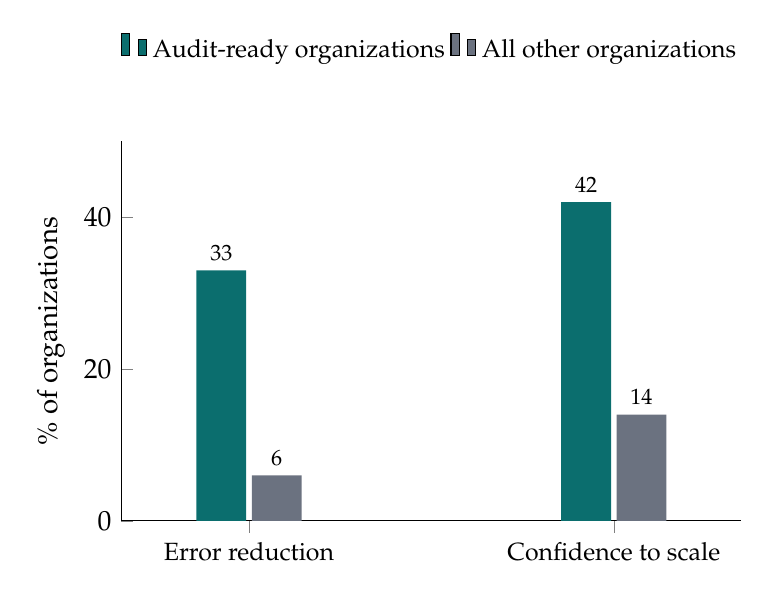
\begin{tikzpicture}
\begin{axis}[
  ybar, bar width=18pt,
  width=0.78\textwidth, height=6.4cm,
  ymin=0, ymax=50,
  ylabel={\% of organizations},
  symbolic x coords={Error reduction, Confidence to scale},
  xtick=data,
  x tick label style={font=\small},
  enlarge x limits=0.35,
  nodes near coords,
  nodes near coords style={font=\footnotesize},
  legend style={at={(0.5,1.18)},anchor=south,legend columns=-1,font=\small,draw=none},
  axis x line*=bottom, axis y line*=left,
]
\addplot[fill=accent, draw=none] coordinates {(Error reduction,33) (Confidence to scale,42)};
\addplot[fill=muted, draw=none] coordinates {(Error reduction,6) (Confidence to scale,14)};
\legend{Audit-ready organizations, All other organizations}
\end{axis}
\end{tikzpicture}
\caption{Outcomes of audit-ready organizations versus the rest. Global data. Source: KPMG, \emph{Global AI in Finance 2026}, via~\cite{kpmgfin}.}
\label{fig:ctrl}
\end{figure}

The Mexican context adds a nuance about the visibility of the cost of AI itself. According to the Global AI Pulse, 43\% of Mexican companies have cost dashboards (53\% globally), 38\% report only partial visibility of AI spending, and 46\% have difficulty understanding cost structures, against one in three globally~\cite{kpmgpulse}. Put differently, before AI can solve the collections problem, the company needs to be able to count what AI itself costs.

There remains the SAT chapter, which the playbook frames with restrained drama. The 16,200 scheduled audits amount to less than 0.03\% of a register of 66.8 million taxpayers, according to one of the sources consulted~\cite{sad}, so the probability of a formal review is low. The relevant exposure, and here the playbook is right, is another: automated detection of discrepancies among what was invoiced, declared, and collected, and the company's ability to reconstruct the file of a transaction. Hence the three tests it proposes: gather ten invoices from eight months ago with their CFDI, their payment complement, and the bank movement that settled them; count how many of last month's payments were applied without manual entry; and estimate how many days it would take to assemble a file in response to a requirement. The tests are cheap, and their result is, by itself, a diagnosis.

\section{The DSO calculation}

The playbook proposes a calculation fit for a committee: divide annual credit sales by 365 to obtain what one day of DSO is worth in cash, multiply it by the cost of capital to obtain the recurring saving, and subtract the total cost of the solution. It rigorously separates the cash released, which occurs once, from the saving, which is recurring, and asks that they be presented separately and after tax.

Table~\ref{tab:dso} extends its example (MXN 1,200 million in credit sales) to three costs of capital. The after-tax values assume a corporate income tax rate of 30\%, an assumption of this reading that each company should replace with its own.

\begin{table}[h]
\centering
\small
\begin{tabular}{@{}rrr@{}}
\toprule
Cost of capital & Annual saving per DSO day & After income tax (30\%) \\
\midrule
8\% & MXN 263,000 & MXN 184,000 \\
12\% & MXN 395,000 & MXN 276,000 \\
16\% & MXN 526,000 & MXN 368,000 \\
\bottomrule
\end{tabular}
\caption{Recurring value of one DSO day with MXN 1,200 million in credit sales. One day equals MXN 3.29 million of cash released once.}
\label{tab:dso}
\end{table}

An example illustrates the scale: cutting DSO by five days releases MXN 16.4 million of cash, once, and at 12\% yields MXN 1.97 million of annual saving before tax, or MXN 1.38 million after. That is the figure to compare against the recurring cost of fees, licenses, and staff hours, not the cash released, which is an event rather than a flow. The playbook's other warning deserves emphasis: DSO must be computed on credit sales, not total sales, because with the latter the number comes out optimistic.

\section{Five practical principles}

The following principles are this reading's own synthesis. They are not claims made by the playbook or by the sources.

\begin{enumerate}[leftmargin=1.6em, itemsep=0.2em]
\item \textbf{Instrument before you buy.} Establishing the baseline for the six metrics (close, reconciliation without manual entry, portfolio risk, DSO by aging bucket, traceability, and hours spent on data entry) requires no vendor. Without it, any later improvement is an anecdote.
\item \textbf{Distinguish the model from the rule.} Ask each solution which of its functions learns and which applies rules, and evaluate each by its own criterion: calibration for the model, automatic application rate and exception handling for the rule.
\item \textbf{Design the audit trail before automating.} Define who authorizes exceptions, what is recorded, and how duties are segregated, and take it to the audit committee before signing.
\item \textbf{Read each figure against its denominator.} Compare your own company with the universe it belongs to, not with the most striking average.
\item \textbf{Verify the rule with whoever answers for it.} In tax matters, distinguish obligation from penalty and confirm dates and rules with a tax advisor before deciding.
\end{enumerate}

As a complement, the five questions with which the playbook invites readers to interrogate a vendor (pricing model, native or custom ERP integration, duration of recent implementations, Mexican references of comparable size including one that ran into problems, and data portability) form a protocol that works for any vendor, not only Paystand. Two additions are suggested, consistent with the document's thesis: which of the six metrics will move and how it will be measured, and what control evidence each automated transaction leaves behind.

\section{Limitations and methodological note}
\label{sec:limits}

This reading contains no original data and uses no data from any client, employer, or company. Its scope is bounded by the following.

\begin{itemize}[leftmargin=1.4em, itemsep=0.2em]
\item \textbf{Secondary sources.} Several figures were checked against specialized press and not against the original document: KPMG's study on AI in finance, the study by Centro M\'exico Digital and UNAM, the details of the SAT's 2026 Master Plan, and the 2026 Miscellaneous Tax Resolution. Before citing them in a formal setting, the primary documents should be consulted, including the Official Gazette (DOF) and the SAT communiqu\'e.
\item \textbf{Unpublished definitions and samples.} KPMG M\'exico's release neither defines ``consolidated return'' nor publishes the Mexican sample size, so the 7\% figure should be read with that reservation.
\item \textbf{Commercial document.} Paystand's own claims (the volume of more than about MXN 400,000 million processed per year, the client list, the integrations, and the testimonials) were not independently verified.
\item \textbf{Associations, not causes.} The five-to-one ratio and the differences between audit-ready and other organizations are reported associations, not demonstrated effects.
\item \textbf{Tax Mailbox date.} The sources consulted do not fully agree. The reading that 2027 marks the start of the penalty is the one supported by the most recent source, and it should be confirmed against the applicable rule.
\item \textbf{Currency conversion.} The sources report revenue thresholds and volumes in U.S. dollars. They are expressed here in pesos using the approximate rate of MXN 20 per dollar implied by the playbook itself (USD 250 million $\approx$ MXN 5,000 million), so they are orders of magnitude and not exact conversions.
\item \textbf{Illustrative calculations.} Table~\ref{tab:dso} uses assumed costs of capital and an assumed income tax rate. It is not tax or financial advice.
\end{itemize}

\section{Conclusion}

Before asking whether the machine thinks, it would be worth knowing whether the house can count. Paystand's playbook, despite its commercial vocation, has the merit of placing the question in the right order: first the measure, then the instrument. The Mexican data confirm that the moment calls for it. A 7\% consolidated return, identical to the world's, indicates that the challenge is not adopting but demonstrating, and that the competitive advantage of the coming years will belong less to whoever buys the most sophisticated tool than to whoever can show, with their own traceable numbers, what changed because of it.

\begin{thebibliography}{99}\small
\bibitem{paystand} Paystand. \emph{El playbook de IA para finanzas que necesitas leer antes de que empiece 2027} (\emph{Playbook de IA para finanzas 2027}), ten-page PDF document, 2026. In Spanish.
\bibitem{kpmgpulse} KPMG M\'exico. ``Las empresas en M\'exico aceleran el uso de IA, pero enfrentan dificultades para demostrar el retorno de la inversi\'on'', press release on the \emph{Global AI Pulse Q2 2026}, 28 July 2026. In Spanish. \url{https://kpmg.com/mx/es/sala-de-prensa/comunicados-de-prensa/2026/07/cp-las-empresas-en-mexico-aceleran-el-uso-de-ia-pero-enfrentan-dificultades-para-demostrar-el-retorno-de-la-inversion.html}
\bibitem{kpmgfin} IT Brief US. ``KPMG finds finance AI use rises to 75\% on governance'', 14 May 2026 (summary of KPMG's \emph{Global AI in Finance 2026} study). \url{https://itbrief.news/story/kpmg-finds-finance-ai-use-rises-to-75-on-governance}
\bibitem{cmd} El Cronista. ``El dilema de la innovaci\'on financiera: el potencial dispara la producci\'on pero su adopci\'on se estanca en 8.4\%'', 6 August 2026 (study by Centro M\'exico Digital and UNAM's Faculty of Engineering). In Spanish. \url{https://www.cronista.com/mexico/finanzas-economia/el-dilema-de-la-innovacion-financiera-el-potencial-dispara-la-produccion-pero-su-adopcion-se-estanca-en-84/}
\bibitem{bl} Bloomberg L\'inea. ``SAT prepara miles de auditor\'ias a contribuyentes con alto riesgo de impago en 2026'', October 2025. In Spanish. \url{https://www.bloomberglinea.com/latinoamerica/mexico/sat-prepara-miles-de-auditorias-a-contribuyentes-con-alto-riesgo-de-impago-en-2026/}
\bibitem{sad} Siempre al D\'ia. ``Plan Maestro 2026 del SAT: gu\'ia sobre lo que el contador debe revisar en cada cliente''. In Spanish. \url{https://siemprealdia.co/mexico/fiscal/plan-maestro-2026-del-sat/}
\bibitem{pwc} PwC M\'exico. ``Inicia una nueva etapa de negociaci\'on para Norteam\'erica'', July 2026. In Spanish. \url{https://www.pwc.com/mx/es/impuestos/novedades-fiscales/nueva-etapa-de-negociacion-tmec-2026.html}
\bibitem{proceso} Proceso. ``Buz\'on Tributario SAT 2026: cu\'al es el plazo para habilitarlo y evitar multas'', 5 October 2026. In Spanish. \url{https://www.proceso.com.mx/economia/2026/10/5/buzon-tributario-sat-2026-cual-es-el-plazo-para-habilitarlo-y-evitar-multas-381245.html}
\bibitem{contrib} El Contribuyente. ``¿Estás en RESICO? Estos cambios obligatorios llegan en 2026'', January 2026. In Spanish. \url{https://www.elcontribuyente.mx/2026/01/estas-en-resico-estos-cambios-obligatorios-llegan-en-2026/}
\bibitem{tokenomics} Tokenomics Foundation. \emph{State of Tokenomics}, Release Candidate 1.0, 23 September 2026. \url{https://www.tokeneconomics.com/state-of-tokenomics/}
\end{thebibliography}

\vfill
\begin{center}
\footnotesize\color{muted}
This reading is independent. It is not affiliated with, or endorsed by, Paystand, KPMG, the SAT, or any other institution cited.
\end{center}

\end{document}
